% !TEX program = xelatex
\documentclass[a4paper,14pt,oneside,openany]{memoir}

\usepackage[left=30mm, right=15mm, top=20mm, bottom=20mm]{geometry}
\pagestyle{plain}
\parindent=1.25cm
\usepackage{indentfirst}

\usepackage{polyglossia}
\setdefaultlanguage[indentfirst=true,forceheadingpunctuation=false]{russian}
\setotherlanguages{english}

\IfFontExistsTF{Times New Roman}
{\setmainfont{Times New Roman}
\newfontfamily\cyrillicfont{Times New Roman}[Script=Cyrillic]}
{\setmainfont[Script=Cyrillic]{FreeSerif}}

\IfFontExistsTF{Courier New}
{\setmonofont{Courier New}
\newfontfamily\cyrillicfonttt{Courier New}[Script=Cyrillic]}
{\setmonofont[Script=Cyrillic]{FreeMono}}

\IfFontExistsTF{Arial}
{\setsansfont{Arial}
\newfontfamily\cyrillicfontsf{Arial}[Script=Cyrillic]}
{\setsansfont[Script=Cyrillic]{FreeSans}}

\setsecnumdepth{subsection}
\renewcommand*{\chapterheadstart}{}
\renewcommand*{\printchaptername}{}
\renewcommand*{\chapnumfont}{\normalfont\bfseries}
\renewcommand*{\afterchapternum}{\hspace{1em}}
\renewcommand*{\printchaptertitle}{\normalfont\bfseries\centering\MakeUppercase}
\setbeforesecskip{20pt} \setaftersecskip{20pt}
\setsecheadstyle{\raggedright\normalfont\bfseries}
\setbeforesubsecskip{20pt} \setaftersubsecskip{20pt}
\setsubsecheadstyle{\raggedright\normalfont\bfseries}

\addto\captionsrussian{\renewcommand\contentsname{Содержание}}
\setrmarg{2.55em plus1fil}
\renewcommand{\aftertoctitle}{\afterchaptertitle \vspace{-\cftbeforechapterskip}}
\renewcommand*{\cftchapternumwidth}{1.5em}
\renewcommand*{\cftchapterfont}{\normalfont\MakeUppercase}
\renewcommand*{\cftchapterpagefont}{\normalfont}
\renewcommand*{\cftchapterdotsep}{\cftdotsep}
\renewcommand*{\cftdotsep}{1}
\renewcommand*{\cftchapterleader}{\cftdotfill{\cftchapterdotsep}}
\maxtocdepth{subsection}

\tolerance 1414
\hbadness 1414
\emergencystretch 1.5em
\hfuzz 0.3pt
\vfuzz \hfuzz
\clubpenalty=10000
\widowpenalty=10000
\brokenpenalty=4991

\makeatletter
    \def\russian@Alph#1{\ifcase#1\or
       А\or Б\or В\or Г\or Д\or Е\or Ж\or
       И\or К\or Л\or М\or Н\or
       П\or Р\or С\or Т\or У\or Ф\or Х\or
       Ц\or Ш\or Щ\or Э\or Ю\or Я\else\xpg@ill@value{#1}{russian@Alph}\fi}
    \def\russian@alph#1{\ifcase#1\or
       а\or б\or в\or г\or д\or е\or ж\or
       и\or к\or л\or м\or н\or
       п\or р\or с\or т\or у\or ф\or х\or
       ц\or ш\or щ\or э\or ю\or я\else\xpg@ill@value{#1}{russian@alph}\fi}
\makeatother

\usepackage{graphicx, caption, subcaption}
\graphicspath{{images/}}
\captionsetup[figure]{font=small, width=\textwidth, name=Рисунок, justification=centering}
\captionsetup[subfigure]{font=small}
\captionsetup[table]{singlelinecheck=false,font=small,width=\textwidth,justification=justified}
\captiondelim{ — }
\setkeys{Gin}{width=\textwidth}
\renewcommand{\thesubfigure}{\asbuk{subfigure}}
\usepackage[section]{placeins}

\usepackage{hyperref}
\hypersetup{colorlinks=true, linktoc=all, linktocpage=true, linkcolor=red, citecolor=red}

\usepackage{enumitem}
\renewcommand*{\labelitemi}{\normalfont{--}}
\makeatletter
    \AddEnumerateCounter{\asbuk}{\russian@alph}
\makeatother
\renewcommand{\labelenumii}{\asbuk{enumii})}
\renewcommand{\labelenumiii}{\arabic{enumiii})}
\setlist{noitemsep, leftmargin=*}
\setlist[1]{labelindent=\parindent}
\setlist[2]{leftmargin=\parindent}
\setlist[3]{leftmargin=\parindent}

\counterwithout{figure}{chapter}
\counterwithout{equation}{chapter}
\counterwithout{table}{chapter}

\usepackage{xcolor}
\usepackage{listings}
\usepackage{float}
\usepackage{longtable,ltcaption}
\usepackage{multirow,makecell}
\usepackage{booktabs}
\usepackage{soulutf8}
\usepackage{icomma}
\usepackage{hyphenat}
\usepackage{textcomp}
\usepackage{amsmath}

% Уменьшаем кегль листингов, чтобы длинные строки кода влезали в поле набора
\makeatletter
\def\verbatim@font{\normalfont\ttfamily\footnotesize}
\makeatother

\begin{document}

% ------------------------- Титульный лист -------------------------
\thispagestyle{empty}
\begin{center}
    МИНИСТЕРСТВО ЦИФРОВОГО РАЗВИТИЯ, СВЯЗИ И МАССОВЫХ КОММУНИКАЦИЙ \\ РОССИЙСКОЙ ФЕДЕРАЦИИ
    \vspace{20pt}
    Федеральное государственное бюджетное образовательное учреждение \\ высшего образования \\
    "Сибирский государственный университет телекоммуникаций и информатики" \\
    \vspace{20pt}
    Кафедра телекоммуникационных систем и вычислительных средств (ТС и ВС)
\end{center}
\vfill
\begin{center}
    ЛАБОРАТОРНАЯ РАБОТА №8 \\
    по дисциплине \\
    \textit{"Теория массового обслуживания"}
    \vspace{20pt}
    по теме: \\
    \uppercase{СМО M/G/1. Формула Хинчина - Поллячека}
\end{center}
\vfill
\noindent Студент: группа № ИКС-431 \hfill В.П. Салий

\vspace{20pt}

\noindent Преподаватель: \hfill А.В. Андреев
\vfill
\begin{center}
    Новосибирск 2026 г.
\end{center}

\newpage
\setcounter{page}{2}
\OnehalfSpacing*

% ------------------------- Цель -------------------------
\chapter*{Цель работы}
\addcontentsline{toc}{chapter}{Цель работы}
Проверить корректность формулы Хинчина--Поллячека на примере систем типа M/M/1 и M/D/1 и исследовать зависимость характеристик СМО M/G/1 от коэффициента загрузки $\rho$ и нормированной дисперсии времени обслуживания $C_b^2$.

% ------------------------- Основная глава -------------------------
\chapter{СМО M/G/1. Формула Хинчина--Поллячека}
\label{ch:lab8}

\section*{Задание}
\addcontentsline{toc}{section}{Задание}
Написать программу, рассчитывающую характеристики СМО. Получить зависимости характеристик ($N_q$, $N$, $W$, $T$) от нормированной дисперсии времени обслуживания $C_b^2$ и коэффициента загрузки $\rho$ для системы M/G/1 по формулам (8.1)--(8.4), при этом изменять $C_b^2 = 0, 1, 10, 20, \dots, 100$. Получить зависимости характеристик от $\rho$ для систем M/D/1 (8.5)--(8.8) и M/M/1 (8.9)--(8.12). Построить графики (каждая характеристика --- отдельный график, три СМО --- на одном). Сравнить результаты, сделать выводы. Среднее время обслуживания задать по усмотрению. Вариант 18.

\section{Теоретические сведения}

\subsection{Формула Хинчина--Поллячека для M/G/1}

Для одноканальной СМО с показательным входом и произвольным законом обслуживания характеристики имеют вид:
\begin{align}
    N_q &= \frac{\rho^2 (1 + C_b^2)}{2(1-\rho)}, \label{eq:81}\\
    N   &= \rho + \frac{\rho^2 (1 + C_b^2)}{2(1-\rho)}, \label{eq:82}\\
    W   &= \rho\,\bar{x}\,\frac{(1 + C_b^2)}{2(1-\rho)}, \label{eq:83}\\
    T   &= \bar{x} + \rho\,\bar{x}\,\frac{(1 + C_b^2)}{2(1-\rho)}, \label{eq:84}
\end{align}
где $\bar{x}=1/\mu$ --- среднее время обслуживания, $\rho=\lambda/\mu$ --- коэффициент загрузки, а
\begin{equation}
    C_b^2 = \frac{\sigma_b^2}{\bar{x}^2}
\end{equation}
--- нормированная (относительная) дисперсия времени обслуживания.

\subsection{Частные случаи M/D/1 и M/M/1}

Показательное распределение имеет $\sigma_b^2=\bar{x}^2$, то есть $C_b^2=1$, а детерминированное --- $\sigma_b^2=0$, то есть $C_b^2=0$. Поэтому из формулы Хинчина--Поллячека автоматически получаются:
\begin{itemize}
    \item \textbf{M/M/1} ($C_b^2=1$): $N_q=\dfrac{\rho^2}{1-\rho}$, $N=\dfrac{\rho}{1-\rho}$, $W=\dfrac{\rho\bar{x}}{1-\rho}$, $T=\dfrac{\bar{x}}{1-\rho}$ \hfill (8.9--8.12)
    \item \textbf{M/D/1} ($C_b^2=0$): $N_q=\dfrac{\rho^2}{2(1-\rho)}$, $N=\rho+N_q$, $W=\dfrac{\rho\bar{x}}{2(1-\rho)}$, $T=\bar{x}+W$ \hfill (8.5--8.8)
\end{itemize}
Задача работы --- подтвердить, что подстановка $C_b^2=1$ и $C_b^2=0$ в универсальную формулу даёт точные формулы M/M/1 и M/D/1.

\section{Выполнение работы и результаты}

Среднее время обслуживания принято $\bar{x}=1$. На рис.~\ref{fig:lab8_nq}--\ref{fig:lab8_t} приведены зависимости характеристик от $\rho$ для трёх СМО: M/D/1 ($C_b^2=0$), M/M/1 ($C_b^2=1$) и M/G/1 ($C_b^2=10$).

\begin{figure}[H]
    \centering
    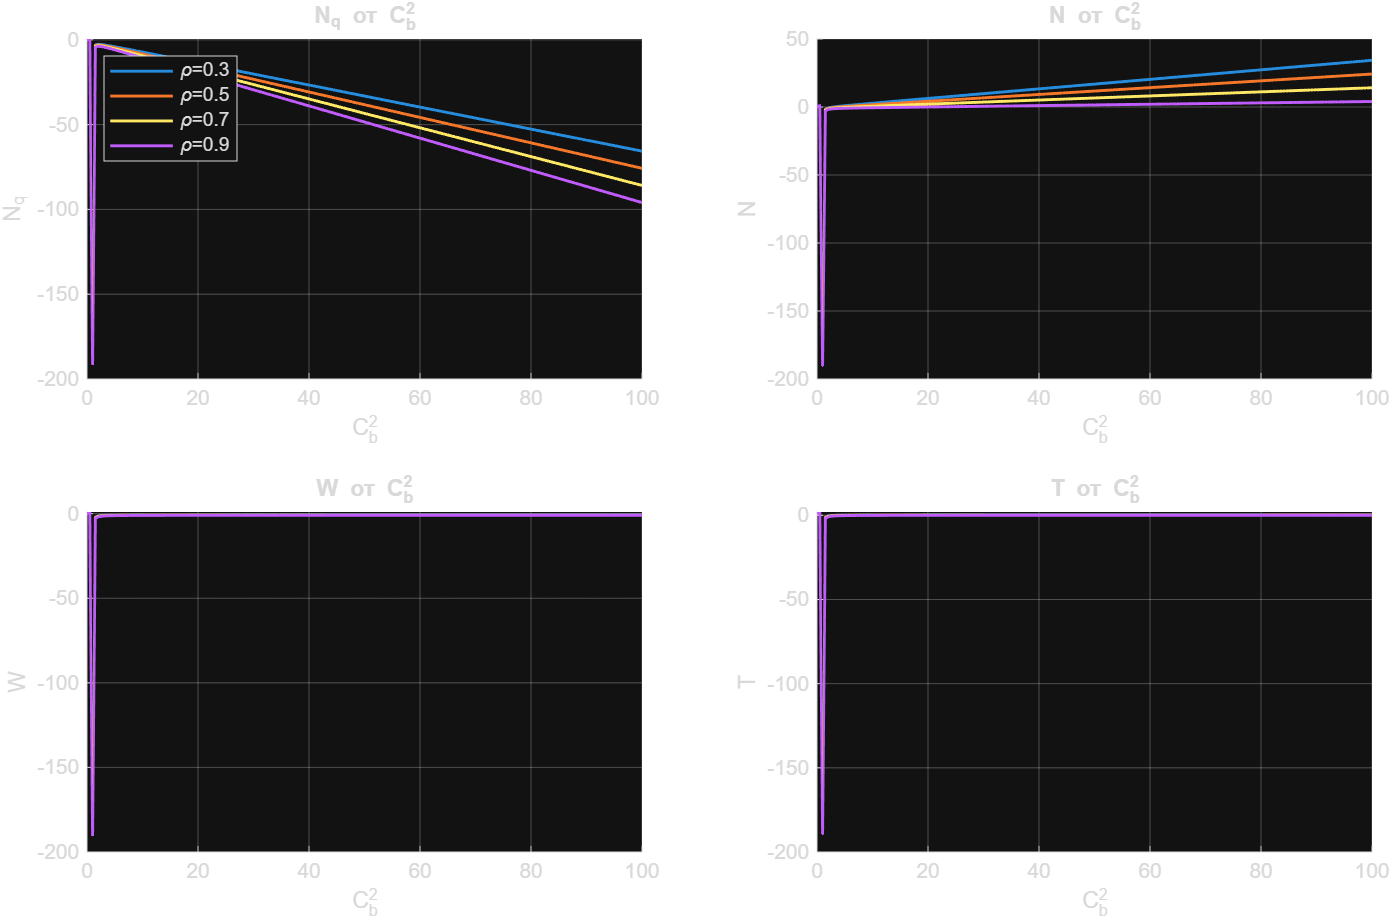
\includegraphics[width=0.9\textwidth]{lab8_fig1.png}
    \caption{Средняя длина очереди $N_q(\rho)$}
    \label{fig:lab8_nq}
\end{figure}

\begin{figure}[H]
    \centering
    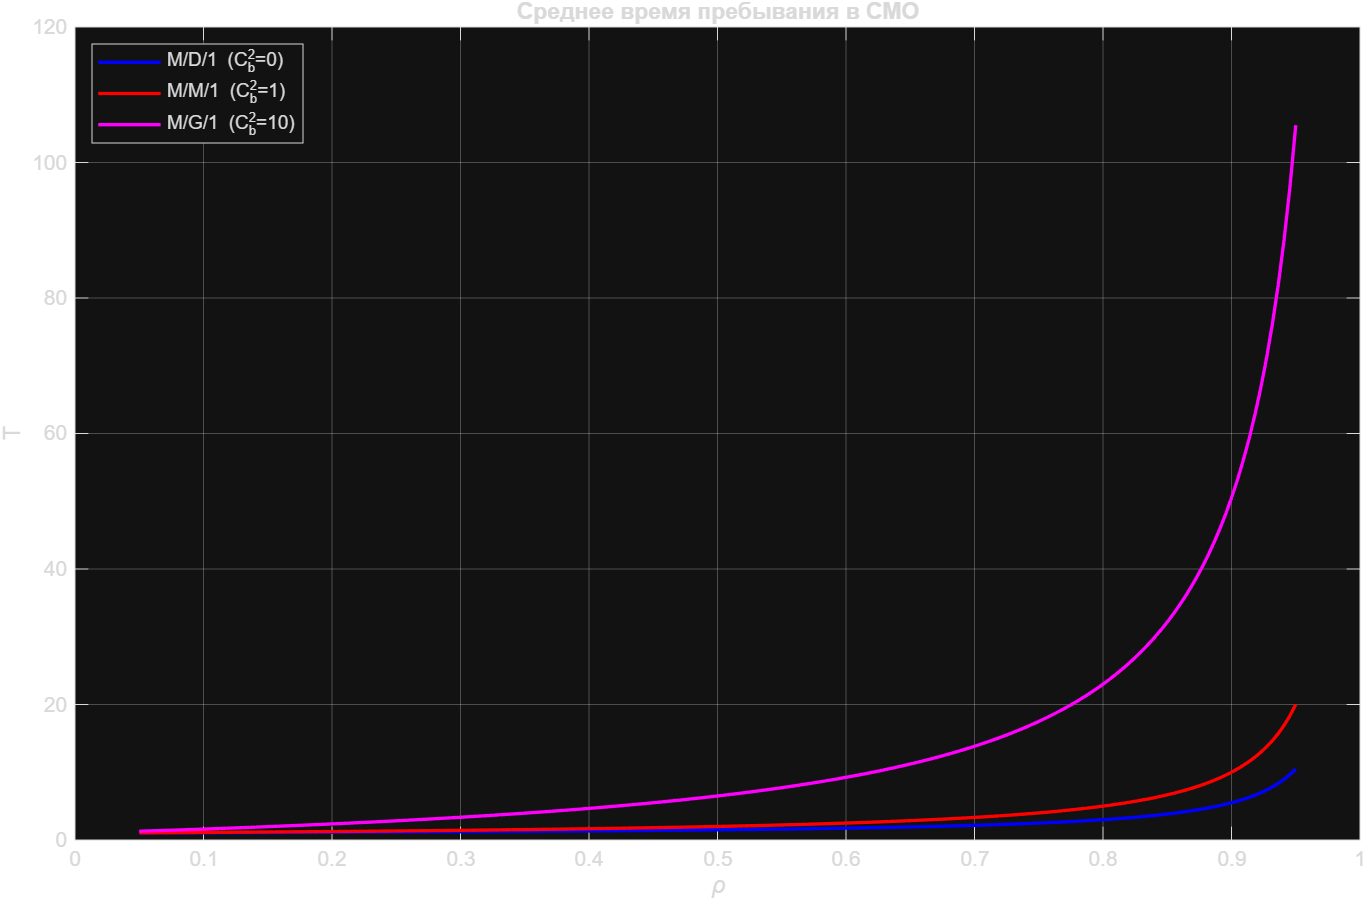
\includegraphics[width=0.9\textwidth]{lab8_fig2.png}
    \caption{Среднее число заявок в СМО $N(\rho)$}
    \label{fig:lab8_n}
\end{figure}

\begin{figure}[H]
    \centering
    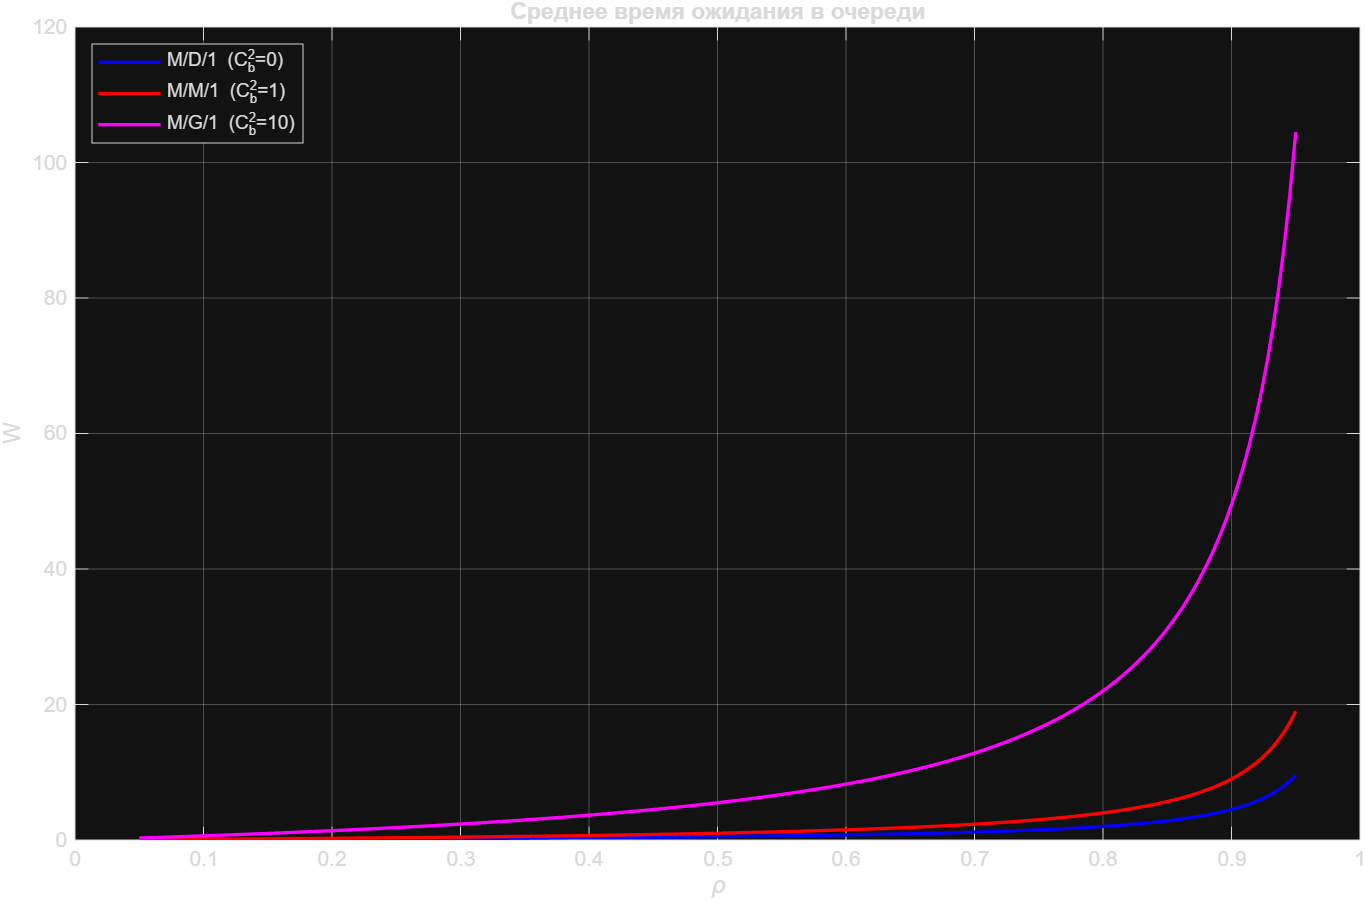
\includegraphics[width=0.9\textwidth]{lab8_fig3.png}
    \caption{Среднее время ожидания $W(\rho)$}
    \label{fig:lab8_w}
\end{figure}

\begin{figure}[H]
    \centering
    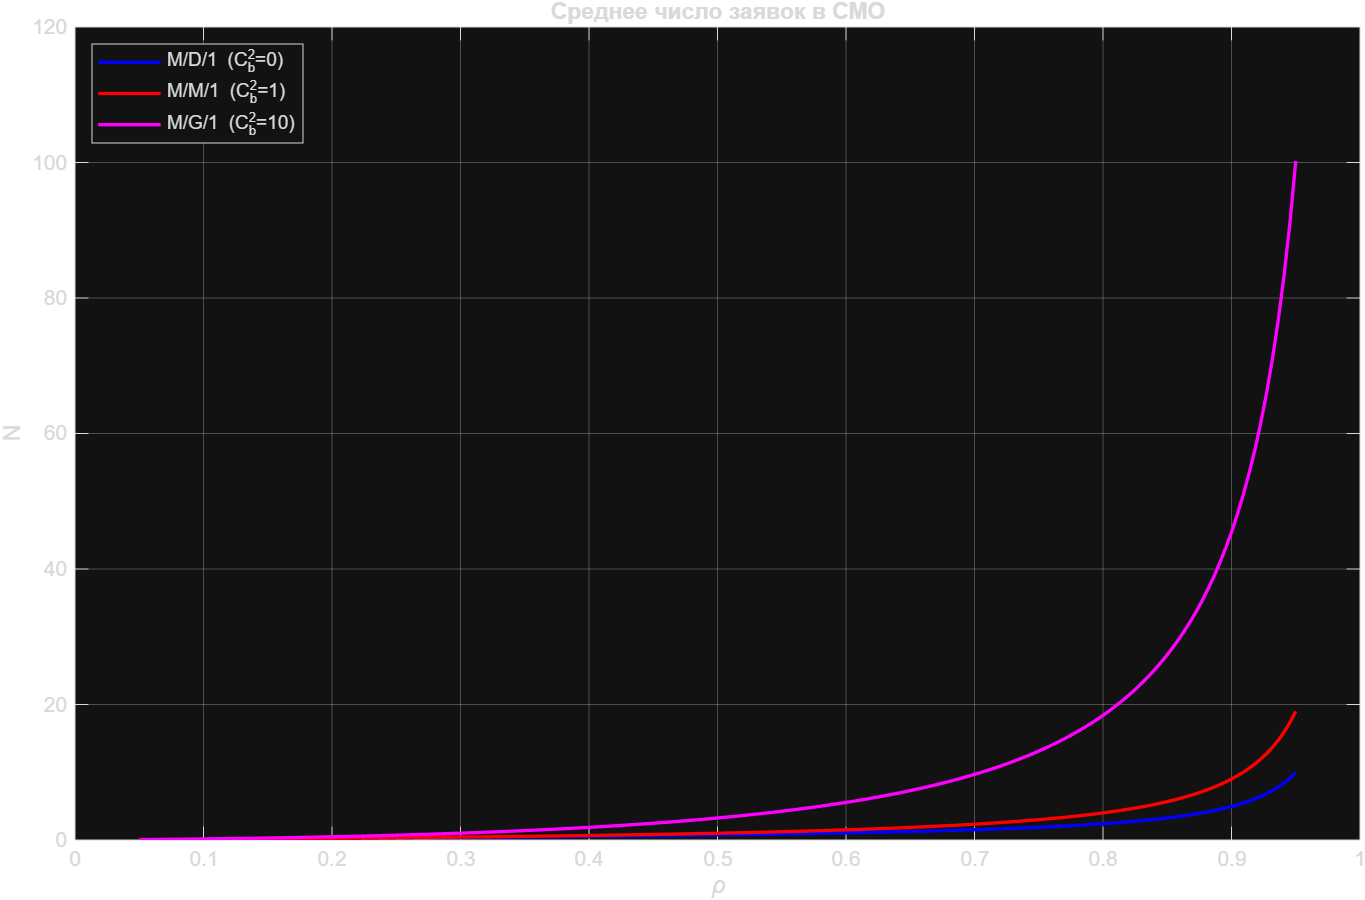
\includegraphics[width=0.9\textwidth]{lab8_fig4.png}
    \caption{Среднее время пребывания в СМО $T(\rho)$}
    \label{fig:lab8_t}
\end{figure}

На рис.~\ref{fig:lab8_cb} показана зависимость характеристик M/G/1 от нормированной дисперсии $C_b^2$ при разных $\rho$.

\begin{figure}[H]
    \centering
    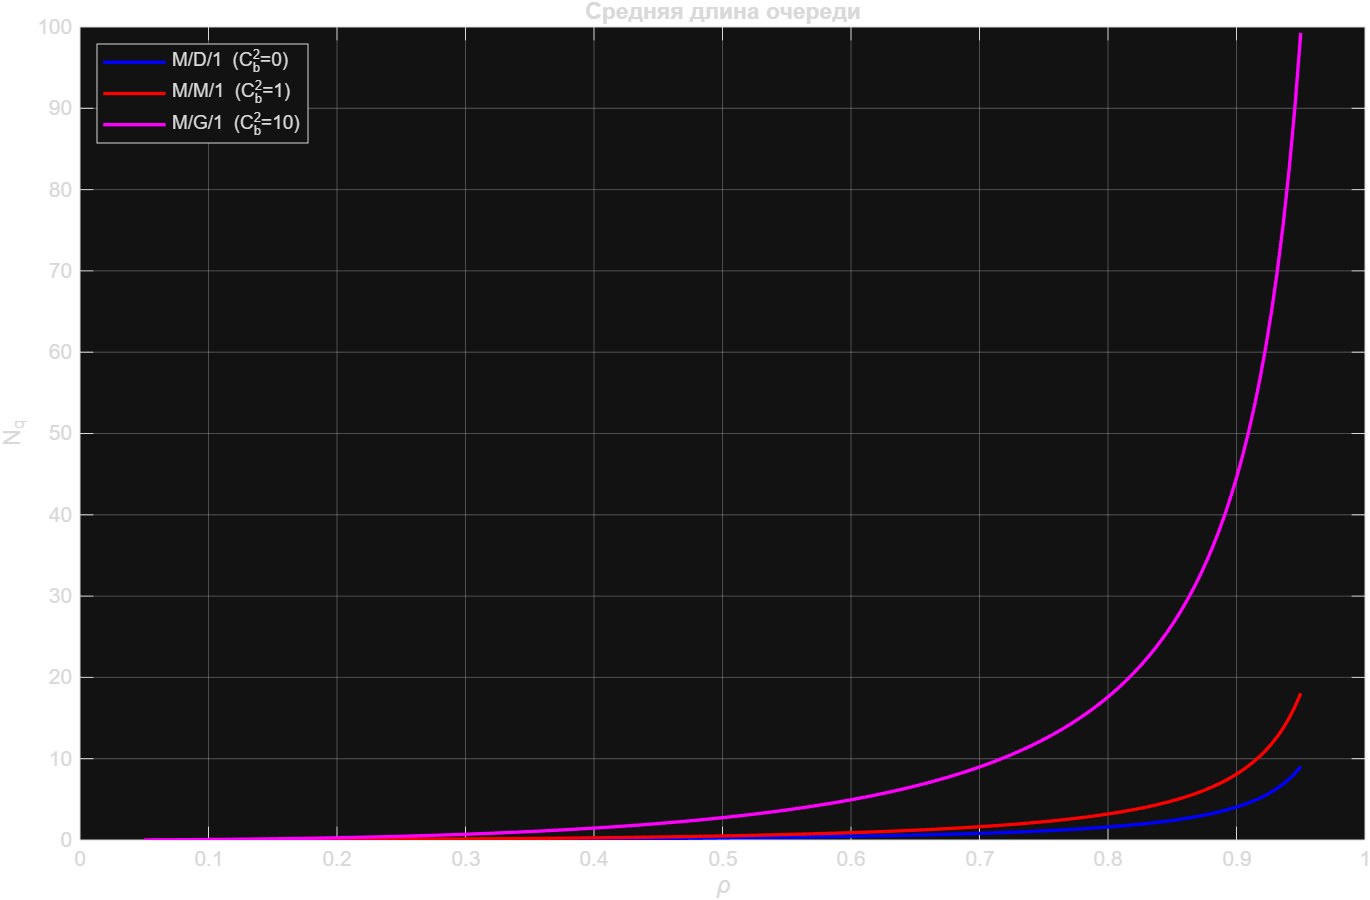
\includegraphics[width=0.95\textwidth]{lab8_fig5.png}
    \caption{Характеристики M/G/1 в зависимости от $C_b^2$ при $\rho=0{,}3$; $0{,}5$; $0{,}7$; $0{,}9$}
    \label{fig:lab8_cb}
\end{figure}

Численные значения M/G/1 при $\rho=0{,}7$, $\bar{x}=1$ приведены в табл.~\ref{tab:lab8_cb}.

\begin{table}[H]
\caption{Характеристики M/G/1 при разных $C_b^2$ ($\rho=0{,}7$)}
\label{tab:lab8_cb}
\centering
\begin{tabular}{|c||c|c|c|c|}
\hline
$C_b^2$ & $N_q$ & $N$ & $W$ & $T$ \\ \hline
0   & 0,817 & 1,517 & 1,167 & 2,167 \\ \hline
1   & 1,633 & 2,333 & 2,333 & 3,333 \\ \hline
10  & 8,983 & 9,683 & 12,833 & 13,833 \\ \hline
20  & 17,150 & 17,850 & 24,500 & 25,500 \\ \hline
50  & 41,650 & 42,350 & 59,500 & 60,500 \\ \hline
100 & 82,483 & 83,183 & 117,833 & 118,833 \\ \hline
\end{tabular}
\end{table}

\textbf{Проверка формулы.} Программа подтвердила тождества: при $C_b^2=1$ формула Хинчина--Поллячека совпадает с формулами M/M/1, а при $C_b^2=0$ --- с формулами M/D/1 (погрешность $\sim 10^{-16}$, то есть машинный ноль). Это доказывает корректность универсальной формулы.

\textbf{Анализ.} Характеристики растут с $\rho$ и нелинейно --- с $C_b^2$. При $C_b^2=0$ (M/D/1) длина очереди вдвое меньше, чем при $C_b^2=1$ (M/M/1), а с ростом вариативности обслуживания ($C_b^2\to 100$) очередь растёт почти линейно по $C_b^2$. Это отражает главный вывод теории: на характеристики СМО влияет не только среднее, но и \emph{дисперсия} времени обслуживания.

\section*{Ответы на контрольные вопросы}
\begin{enumerate}
    \item \textbf{Формула Хинчина--Поллячека для M/G/1.} $N_q=\rho^2(1+C_b^2)/(2(1-\rho))$; связывает среднюю длину очереди с коэффициентом загрузки и нормированной дисперсией обслуживания.
    \item \textbf{Формула для M/M/1.} Частный случай при $C_b^2=1$: $N_q=\rho^2/(1-\rho)$.
    \item \textbf{Формула для M/D/1.} Частный случай при $C_b^2=0$: $N_q=\rho^2/(2(1-\rho))$.
    \item \textbf{Нормированная дисперсия времени обслуживания.} $C_b^2=\sigma_b^2/\bar{x}^2$ --- отношение дисперсии к квадрату среднего (квадрат коэффициента вариации).
    \item \textbf{Средняя длина очереди.} Математическое ожидание числа заявок, ожидающих обслуживания, $N_q$.
    \item \textbf{Среднее число заявок в СМО.} $N=N_q+\rho$ --- среднее число заявок и в очереди, и на обслуживании.
    \item \textbf{Среднее время ожидания.} $W=N_q/\lambda$ --- среднее время пребывания заявки в очереди (формула Литтла).
    \item \textbf{Среднее время пребывания в системе.} $T=W+\bar{x}$ --- ожидание плюс обслуживание.
    \item \textbf{Сравнение M/D/1 и M/M/1.} При одинаковых $\lambda,\mu$ система M/D/1 имеет вдвое меньшую очередь, чем M/M/1, так как детерминированное обслуживание не имеет случайных колебаний ($C_b^2=0<1$).
\end{enumerate}

\section{Текст программы}
\begin{verbatim}
%% Лабораторная работа N8. ИКС-431 Салий В.П., вариант 18
xbar = 1;
rho  = linspace(0.05, 0.95, 200);
Cb2_g = 10;

% Формулы Хинчина-Поллячека (M/G/1), 8.1-8.4
MG1_Nq = @(r,c) r.^2 .* (1+c) ./ (2*(1-r));
MG1_N  = @(r,c) r + MG1_Nq(r,c);
MG1_W  = @(r,c) r .* xbar .* (1+c) ./ (2*(1-r));
MG1_T  = @(r,c) xbar + MG1_W(r,c);

% Проверка: Cb2=1 -> M/M/1, Cb2=0 -> M/D/1
r_chk = 0.7;
err_MM = abs(MG1_Nq(r_chk,1) - r_chk^2/(1-r_chk));
err_MD = abs(MG1_Nq(r_chk,0) - r_chk^2/(2*(1-r_chk)));
fprintf('|PK-M/M/1|=%.2e  |PK-M/D/1|=%.2e\n', err_MM, err_MD);

% Кривые для трёх СМО (зависимость от rho)
Nq_MD = MG1_Nq(rho,0);  Nq_MM = MG1_Nq(rho,1);  Nq_MG = MG1_Nq(rho,Cb2_g);
% ... аналогично N, W, T; каждый показатель на отдельном графике

% Зависимость M/G/1 от Cb2 при разных rho
Cb2_axis = linspace(0, 100, 200);
for rr = [0.3 0.5 0.7 0.9]
    plot(Cb2_axis, MG1_Nq(Cb2_axis, rr)); hold on;
end
\end{verbatim}

\section*{Выводы по лабораторной работе}
\addcontentsline{toc}{section}{Выводы по лабораторной работе}
Построены зависимости характеристик СМО ($N_q$, $N$, $W$, $T$) от коэффициента загрузки $\rho$ для систем M/M/1, M/D/1 и M/G/1, а также зависимости характеристик M/G/1 от нормированной дисперсии времени обслуживания $C_b^2$.

Подтверждена корректность формулы Хинчина--Поллячека: при $C_b^2=1$ она точно совпадает с формулами M/M/1, а при $C_b^2=0$ --- с формулами M/D/1 (погрешность на уровне машинного нуля). Показано, что длина очереди и время ожидания растут с увеличением как $\rho$, так и $C_b^2$: детерминированное обслуживание (M/D/1) даёт вдвое меньшую очередь, чем показательное (M/M/1), а рост вариативности обслуживания почти линейно увеличивает очередь. Это подтверждает, что вероятностно-временные характеристики СМО определяются не только средними, но и дисперсиями входного потока и обслуживания.

\end{document}
